\chapter{Aufgabe D3 und D4}

\section{Simulink-Modell}
Die nachfolgenden Abbildungen zeigen das Simulink-Modell zur Berechnung der Distanz der einzelnen Räder.\\
Das erste Modell in \autoref{fig:TireSimRandomMain} hat die vier Geschwindigkeiten (in m/s) der Räder als Eingänge. Diese werden integriert, um die Strecke zu erhalten. An den Transport Delay Gliedern wurde ein Time Delay von 10 eingestellt. Anschließend wird das verschobene Signal von der wirklichen Strecke abgezogen, damit immer nur ein Zeitraum von 10s betrachtet wird. Die Strecke in dieser Zeitspanne wird von allen vier Rädern verwendet, um den Durchschnitt zu berechnen. Anschließend wird für jedes Rad berechnet, wie weit die Strecke vom Durchschnitt abweicht. Bei einer Abweichung von mehr als 0,05\% liegt die Kurve im Scope bei "1", sonst bei "0".

\begin{figure}[h!]
	\centering
	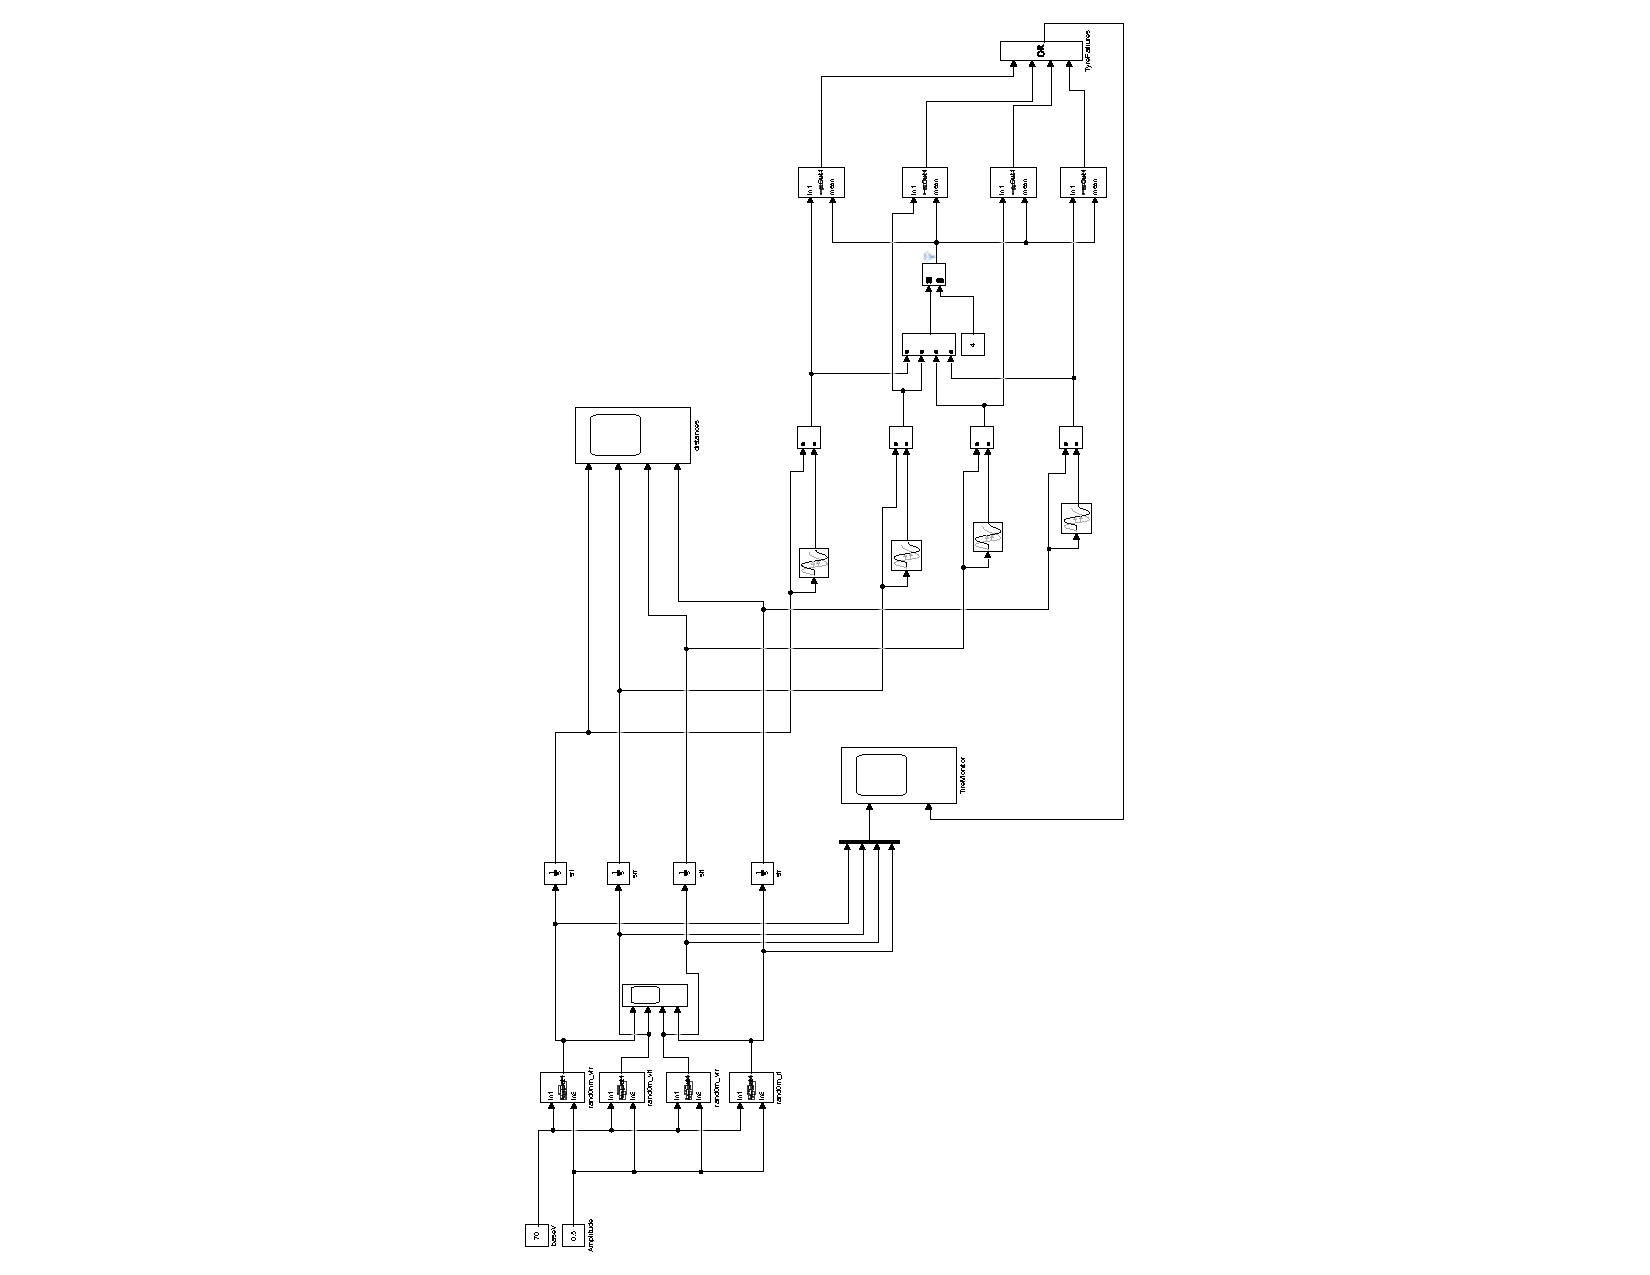
\includegraphics[height=0.95\textheight]{../Graphiken/TireSimRandomMain.pdf}
	\caption{Simulink-Modell1}
	\label{fig:TireSimRandomMain}
\end{figure}

\begin{figure}
	\centering
	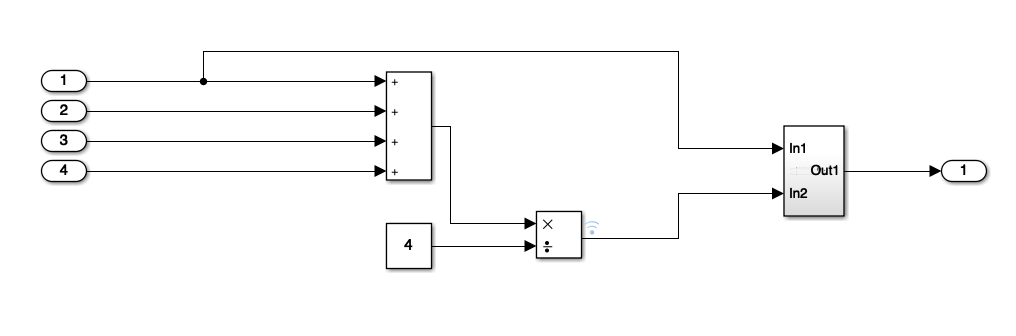
\includegraphics[width=1\linewidth]{../Graphiken/Simulink2}
	\caption{Subsysteme des Simulink-Modell1}
	\label{fig:Simulink2}
\end{figure}

\begin{figure}
	\centering
	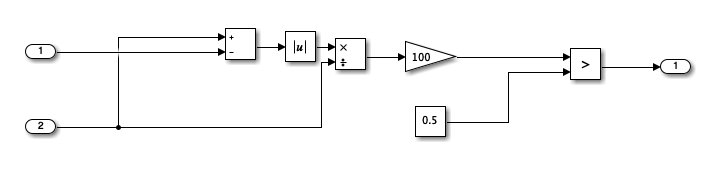
\includegraphics[width=1\linewidth]{../Graphiken/Simulink3}
	\caption{Subsysteme des Simulink-Modell2}
	\label{fig:Simulink3}
\end{figure}

\begin{figure}
	\centering
	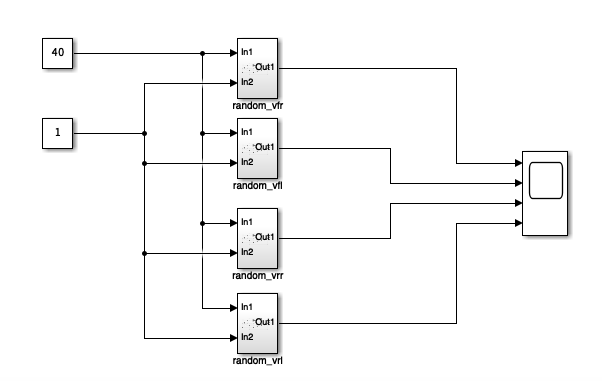
\includegraphics[width=1\linewidth]{../Graphiken/Simulink4}
	\caption{Subsysteme des Simulink-Modell4}
	\label{fig:Simulink4}
\end{figure}





	
	

	
	
	
	